\documentclass[10pt]{article}
\usepackage{tmlr}
% \usepackage[accepted]{tmlr}   % camera-ready
% \usepackage[preprint]{tmlr}   % arXiv
%%%%% NEW MATH DEFINITIONS %%%%%

\usepackage{amsmath,amsfonts,bm}

% Mark sections of captions for referring to divisions of figures
\newcommand{\figleft}{{\em (Left)}}
\newcommand{\figcenter}{{\em (Center)}}
\newcommand{\figright}{{\em (Right)}}
\newcommand{\figtop}{{\em (Top)}}
\newcommand{\figbottom}{{\em (Bottom)}}
\newcommand{\captiona}{{\em (a)}}
\newcommand{\captionb}{{\em (b)}}
\newcommand{\captionc}{{\em (c)}}
\newcommand{\captiond}{{\em (d)}}

% Highlight a newly defined term
\newcommand{\newterm}[1]{{\bf #1}}


% Figure reference, lower-case.
\def\figref#1{figure~\ref{#1}}
% Figure reference, capital. For start of sentence
\def\Figref#1{Figure~\ref{#1}}
\def\twofigref#1#2{figures \ref{#1} and \ref{#2}}
\def\quadfigref#1#2#3#4{figures \ref{#1}, \ref{#2}, \ref{#3} and \ref{#4}}
% Section reference, lower-case.
\def\secref#1{section~\ref{#1}}
% Section reference, capital.
\def\Secref#1{Section~\ref{#1}}
% Reference to two sections.
\def\twosecrefs#1#2{sections \ref{#1} and \ref{#2}}
% Reference to three sections.
\def\secrefs#1#2#3{sections \ref{#1}, \ref{#2} and \ref{#3}}
% Reference to an equation, lower-case.
\def\eqref#1{equation~\ref{#1}}
% Reference to an equation, upper case
\def\Eqref#1{Equation~\ref{#1}}
% A raw reference to an equation---avoid using if possible
\def\plaineqref#1{\ref{#1}}
% Reference to a chapter, lower-case.
\def\chapref#1{chapter~\ref{#1}}
% Reference to an equation, upper case.
\def\Chapref#1{Chapter~\ref{#1}}
% Reference to a range of chapters
\def\rangechapref#1#2{chapters\ref{#1}--\ref{#2}}
% Reference to an algorithm, lower-case.
\def\algref#1{algorithm~\ref{#1}}
% Reference to an algorithm, upper case.
\def\Algref#1{Algorithm~\ref{#1}}
\def\twoalgref#1#2{algorithms \ref{#1} and \ref{#2}}
\def\Twoalgref#1#2{Algorithms \ref{#1} and \ref{#2}}
% Reference to a part, lower case
\def\partref#1{part~\ref{#1}}
% Reference to a part, upper case
\def\Partref#1{Part~\ref{#1}}
\def\twopartref#1#2{parts \ref{#1} and \ref{#2}}

\def\ceil#1{\lceil #1 \rceil}
\def\floor#1{\lfloor #1 \rfloor}
\def\1{\bm{1}}
\newcommand{\train}{\mathcal{D}}
\newcommand{\valid}{\mathcal{D_{\mathrm{valid}}}}
\newcommand{\test}{\mathcal{D_{\mathrm{test}}}}

\def\eps{{\epsilon}}


% Random variables
\def\reta{{\textnormal{$\eta$}}}
\def\ra{{\textnormal{a}}}
\def\rb{{\textnormal{b}}}
\def\rc{{\textnormal{c}}}
\def\rd{{\textnormal{d}}}
\def\re{{\textnormal{e}}}
\def\rf{{\textnormal{f}}}
\def\rg{{\textnormal{g}}}
\def\rh{{\textnormal{h}}}
\def\ri{{\textnormal{i}}}
\def\rj{{\textnormal{j}}}
\def\rk{{\textnormal{k}}}
\def\rl{{\textnormal{l}}}
% rm is already a command, just don't name any random variables m
\def\rn{{\textnormal{n}}}
\def\ro{{\textnormal{o}}}
\def\rp{{\textnormal{p}}}
\def\rq{{\textnormal{q}}}
\def\rr{{\textnormal{r}}}
\def\rs{{\textnormal{s}}}
\def\rt{{\textnormal{t}}}
\def\ru{{\textnormal{u}}}
\def\rv{{\textnormal{v}}}
\def\rw{{\textnormal{w}}}
\def\rx{{\textnormal{x}}}
\def\ry{{\textnormal{y}}}
\def\rz{{\textnormal{z}}}

% Random vectors
\def\rvepsilon{{\mathbf{\epsilon}}}
\def\rvtheta{{\mathbf{\theta}}}
\def\rva{{\mathbf{a}}}
\def\rvb{{\mathbf{b}}}
\def\rvc{{\mathbf{c}}}
\def\rvd{{\mathbf{d}}}
\def\rve{{\mathbf{e}}}
\def\rvf{{\mathbf{f}}}
\def\rvg{{\mathbf{g}}}
\def\rvh{{\mathbf{h}}}
\def\rvu{{\mathbf{i}}}
\def\rvj{{\mathbf{j}}}
\def\rvk{{\mathbf{k}}}
\def\rvl{{\mathbf{l}}}
\def\rvm{{\mathbf{m}}}
\def\rvn{{\mathbf{n}}}
\def\rvo{{\mathbf{o}}}
\def\rvp{{\mathbf{p}}}
\def\rvq{{\mathbf{q}}}
\def\rvr{{\mathbf{r}}}
\def\rvs{{\mathbf{s}}}
\def\rvt{{\mathbf{t}}}
\def\rvu{{\mathbf{u}}}
\def\rvv{{\mathbf{v}}}
\def\rvw{{\mathbf{w}}}
\def\rvx{{\mathbf{x}}}
\def\rvy{{\mathbf{y}}}
\def\rvz{{\mathbf{z}}}

% Elements of random vectors
\def\erva{{\textnormal{a}}}
\def\ervb{{\textnormal{b}}}
\def\ervc{{\textnormal{c}}}
\def\ervd{{\textnormal{d}}}
\def\erve{{\textnormal{e}}}
\def\ervf{{\textnormal{f}}}
\def\ervg{{\textnormal{g}}}
\def\ervh{{\textnormal{h}}}
\def\ervi{{\textnormal{i}}}
\def\ervj{{\textnormal{j}}}
\def\ervk{{\textnormal{k}}}
\def\ervl{{\textnormal{l}}}
\def\ervm{{\textnormal{m}}}
\def\ervn{{\textnormal{n}}}
\def\ervo{{\textnormal{o}}}
\def\ervp{{\textnormal{p}}}
\def\ervq{{\textnormal{q}}}
\def\ervr{{\textnormal{r}}}
\def\ervs{{\textnormal{s}}}
\def\ervt{{\textnormal{t}}}
\def\ervu{{\textnormal{u}}}
\def\ervv{{\textnormal{v}}}
\def\ervw{{\textnormal{w}}}
\def\ervx{{\textnormal{x}}}
\def\ervy{{\textnormal{y}}}
\def\ervz{{\textnormal{z}}}

% Random matrices
\def\rmA{{\mathbf{A}}}
\def\rmB{{\mathbf{B}}}
\def\rmC{{\mathbf{C}}}
\def\rmD{{\mathbf{D}}}
\def\rmE{{\mathbf{E}}}
\def\rmF{{\mathbf{F}}}
\def\rmG{{\mathbf{G}}}
\def\rmH{{\mathbf{H}}}
\def\rmI{{\mathbf{I}}}
\def\rmJ{{\mathbf{J}}}
\def\rmK{{\mathbf{K}}}
\def\rmL{{\mathbf{L}}}
\def\rmM{{\mathbf{M}}}
\def\rmN{{\mathbf{N}}}
\def\rmO{{\mathbf{O}}}
\def\rmP{{\mathbf{P}}}
\def\rmQ{{\mathbf{Q}}}
\def\rmR{{\mathbf{R}}}
\def\rmS{{\mathbf{S}}}
\def\rmT{{\mathbf{T}}}
\def\rmU{{\mathbf{U}}}
\def\rmV{{\mathbf{V}}}
\def\rmW{{\mathbf{W}}}
\def\rmX{{\mathbf{X}}}
\def\rmY{{\mathbf{Y}}}
\def\rmZ{{\mathbf{Z}}}

% Elements of random matrices
\def\ermA{{\textnormal{A}}}
\def\ermB{{\textnormal{B}}}
\def\ermC{{\textnormal{C}}}
\def\ermD{{\textnormal{D}}}
\def\ermE{{\textnormal{E}}}
\def\ermF{{\textnormal{F}}}
\def\ermG{{\textnormal{G}}}
\def\ermH{{\textnormal{H}}}
\def\ermI{{\textnormal{I}}}
\def\ermJ{{\textnormal{J}}}
\def\ermK{{\textnormal{K}}}
\def\ermL{{\textnormal{L}}}
\def\ermM{{\textnormal{M}}}
\def\ermN{{\textnormal{N}}}
\def\ermO{{\textnormal{O}}}
\def\ermP{{\textnormal{P}}}
\def\ermQ{{\textnormal{Q}}}
\def\ermR{{\textnormal{R}}}
\def\ermS{{\textnormal{S}}}
\def\ermT{{\textnormal{T}}}
\def\ermU{{\textnormal{U}}}
\def\ermV{{\textnormal{V}}}
\def\ermW{{\textnormal{W}}}
\def\ermX{{\textnormal{X}}}
\def\ermY{{\textnormal{Y}}}
\def\ermZ{{\textnormal{Z}}}

% Vectors
\def\vzero{{\bm{0}}}
\def\vone{{\bm{1}}}
\def\vmu{{\bm{\mu}}}
\def\vtheta{{\bm{\theta}}}
\def\va{{\bm{a}}}
\def\vb{{\bm{b}}}
\def\vc{{\bm{c}}}
\def\vd{{\bm{d}}}
\def\ve{{\bm{e}}}
\def\vf{{\bm{f}}}
\def\vg{{\bm{g}}}
\def\vh{{\bm{h}}}
\def\vi{{\bm{i}}}
\def\vj{{\bm{j}}}
\def\vk{{\bm{k}}}
\def\vl{{\bm{l}}}
\def\vm{{\bm{m}}}
\def\vn{{\bm{n}}}
\def\vo{{\bm{o}}}
\def\vp{{\bm{p}}}
\def\vq{{\bm{q}}}
\def\vr{{\bm{r}}}
\def\vs{{\bm{s}}}
\def\vt{{\bm{t}}}
\def\vu{{\bm{u}}}
\def\vv{{\bm{v}}}
\def\vw{{\bm{w}}}
\def\vx{{\bm{x}}}
\def\vy{{\bm{y}}}
\def\vz{{\bm{z}}}

% Elements of vectors
\def\evalpha{{\alpha}}
\def\evbeta{{\beta}}
\def\evepsilon{{\epsilon}}
\def\evlambda{{\lambda}}
\def\evomega{{\omega}}
\def\evmu{{\mu}}
\def\evpsi{{\psi}}
\def\evsigma{{\sigma}}
\def\evtheta{{\theta}}
\def\eva{{a}}
\def\evb{{b}}
\def\evc{{c}}
\def\evd{{d}}
\def\eve{{e}}
\def\evf{{f}}
\def\evg{{g}}
\def\evh{{h}}
\def\evi{{i}}
\def\evj{{j}}
\def\evk{{k}}
\def\evl{{l}}
\def\evm{{m}}
\def\evn{{n}}
\def\evo{{o}}
\def\evp{{p}}
\def\evq{{q}}
\def\evr{{r}}
\def\evs{{s}}
\def\evt{{t}}
\def\evu{{u}}
\def\evv{{v}}
\def\evw{{w}}
\def\evx{{x}}
\def\evy{{y}}
\def\evz{{z}}

% Matrix
\def\mA{{\bm{A}}}
\def\mB{{\bm{B}}}
\def\mC{{\bm{C}}}
\def\mD{{\bm{D}}}
\def\mE{{\bm{E}}}
\def\mF{{\bm{F}}}
\def\mG{{\bm{G}}}
\def\mH{{\bm{H}}}
\def\mI{{\bm{I}}}
\def\mJ{{\bm{J}}}
\def\mK{{\bm{K}}}
\def\mL{{\bm{L}}}
\def\mM{{\bm{M}}}
\def\mN{{\bm{N}}}
\def\mO{{\bm{O}}}
\def\mP{{\bm{P}}}
\def\mQ{{\bm{Q}}}
\def\mR{{\bm{R}}}
\def\mS{{\bm{S}}}
\def\mT{{\bm{T}}}
\def\mU{{\bm{U}}}
\def\mV{{\bm{V}}}
\def\mW{{\bm{W}}}
\def\mX{{\bm{X}}}
\def\mY{{\bm{Y}}}
\def\mZ{{\bm{Z}}}
\def\mBeta{{\bm{\beta}}}
\def\mPhi{{\bm{\Phi}}}
\def\mLambda{{\bm{\Lambda}}}
\def\mSigma{{\bm{\Sigma}}}

% Tensor
\DeclareMathAlphabet{\mathsfit}{\encodingdefault}{\sfdefault}{m}{sl}
\SetMathAlphabet{\mathsfit}{bold}{\encodingdefault}{\sfdefault}{bx}{n}
\newcommand{\tens}[1]{\bm{\mathsfit{#1}}}
\def\tA{{\tens{A}}}
\def\tB{{\tens{B}}}
\def\tC{{\tens{C}}}
\def\tD{{\tens{D}}}
\def\tE{{\tens{E}}}
\def\tF{{\tens{F}}}
\def\tG{{\tens{G}}}
\def\tH{{\tens{H}}}
\def\tI{{\tens{I}}}
\def\tJ{{\tens{J}}}
\def\tK{{\tens{K}}}
\def\tL{{\tens{L}}}
\def\tM{{\tens{M}}}
\def\tN{{\tens{N}}}
\def\tO{{\tens{O}}}
\def\tP{{\tens{P}}}
\def\tQ{{\tens{Q}}}
\def\tR{{\tens{R}}}
\def\tS{{\tens{S}}}
\def\tT{{\tens{T}}}
\def\tU{{\tens{U}}}
\def\tV{{\tens{V}}}
\def\tW{{\tens{W}}}
\def\tX{{\tens{X}}}
\def\tY{{\tens{Y}}}
\def\tZ{{\tens{Z}}}


% Graph
\def\gA{{\mathcal{A}}}
\def\gB{{\mathcal{B}}}
\def\gC{{\mathcal{C}}}
\def\gD{{\mathcal{D}}}
\def\gE{{\mathcal{E}}}
\def\gF{{\mathcal{F}}}
\def\gG{{\mathcal{G}}}
\def\gH{{\mathcal{H}}}
\def\gI{{\mathcal{I}}}
\def\gJ{{\mathcal{J}}}
\def\gK{{\mathcal{K}}}
\def\gL{{\mathcal{L}}}
\def\gM{{\mathcal{M}}}
\def\gN{{\mathcal{N}}}
\def\gO{{\mathcal{O}}}
\def\gP{{\mathcal{P}}}
\def\gQ{{\mathcal{Q}}}
\def\gR{{\mathcal{R}}}
\def\gS{{\mathcal{S}}}
\def\gT{{\mathcal{T}}}
\def\gU{{\mathcal{U}}}
\def\gV{{\mathcal{V}}}
\def\gW{{\mathcal{W}}}
\def\gX{{\mathcal{X}}}
\def\gY{{\mathcal{Y}}}
\def\gZ{{\mathcal{Z}}}

% Sets
\def\sA{{\mathbb{A}}}
\def\sB{{\mathbb{B}}}
\def\sC{{\mathbb{C}}}
\def\sD{{\mathbb{D}}}
% Don't use a set called E, because this would be the same as our symbol
% for expectation.
\def\sF{{\mathbb{F}}}
\def\sG{{\mathbb{G}}}
\def\sH{{\mathbb{H}}}
\def\sI{{\mathbb{I}}}
\def\sJ{{\mathbb{J}}}
\def\sK{{\mathbb{K}}}
\def\sL{{\mathbb{L}}}
\def\sM{{\mathbb{M}}}
\def\sN{{\mathbb{N}}}
\def\sO{{\mathbb{O}}}
\def\sP{{\mathbb{P}}}
\def\sQ{{\mathbb{Q}}}
\def\sR{{\mathbb{R}}}
\def\sS{{\mathbb{S}}}
\def\sT{{\mathbb{T}}}
\def\sU{{\mathbb{U}}}
\def\sV{{\mathbb{V}}}
\def\sW{{\mathbb{W}}}
\def\sX{{\mathbb{X}}}
\def\sY{{\mathbb{Y}}}
\def\sZ{{\mathbb{Z}}}

% Entries of a matrix
\def\emLambda{{\Lambda}}
\def\emA{{A}}
\def\emB{{B}}
\def\emC{{C}}
\def\emD{{D}}
\def\emE{{E}}
\def\emF{{F}}
\def\emG{{G}}
\def\emH{{H}}
\def\emI{{I}}
\def\emJ{{J}}
\def\emK{{K}}
\def\emL{{L}}
\def\emM{{M}}
\def\emN{{N}}
\def\emO{{O}}
\def\emP{{P}}
\def\emQ{{Q}}
\def\emR{{R}}
\def\emS{{S}}
\def\emT{{T}}
\def\emU{{U}}
\def\emV{{V}}
\def\emW{{W}}
\def\emX{{X}}
\def\emY{{Y}}
\def\emZ{{Z}}
\def\emSigma{{\Sigma}}

% entries of a tensor
% Same font as tensor, without \bm wrapper
\newcommand{\etens}[1]{\mathsfit{#1}}
\def\etLambda{{\etens{\Lambda}}}
\def\etA{{\etens{A}}}
\def\etB{{\etens{B}}}
\def\etC{{\etens{C}}}
\def\etD{{\etens{D}}}
\def\etE{{\etens{E}}}
\def\etF{{\etens{F}}}
\def\etG{{\etens{G}}}
\def\etH{{\etens{H}}}
\def\etI{{\etens{I}}}
\def\etJ{{\etens{J}}}
\def\etK{{\etens{K}}}
\def\etL{{\etens{L}}}
\def\etM{{\etens{M}}}
\def\etN{{\etens{N}}}
\def\etO{{\etens{O}}}
\def\etP{{\etens{P}}}
\def\etQ{{\etens{Q}}}
\def\etR{{\etens{R}}}
\def\etS{{\etens{S}}}
\def\etT{{\etens{T}}}
\def\etU{{\etens{U}}}
\def\etV{{\etens{V}}}
\def\etW{{\etens{W}}}
\def\etX{{\etens{X}}}
\def\etY{{\etens{Y}}}
\def\etZ{{\etens{Z}}}

% The true underlying data generating distribution
\newcommand{\pdata}{p_{\rm{data}}}
% The empirical distribution defined by the training set
\newcommand{\ptrain}{\hat{p}_{\rm{data}}}
\newcommand{\Ptrain}{\hat{P}_{\rm{data}}}
% The model distribution
\newcommand{\pmodel}{p_{\rm{model}}}
\newcommand{\Pmodel}{P_{\rm{model}}}
\newcommand{\ptildemodel}{\tilde{p}_{\rm{model}}}
% Stochastic autoencoder distributions
\newcommand{\pencode}{p_{\rm{encoder}}}
\newcommand{\pdecode}{p_{\rm{decoder}}}
\newcommand{\precons}{p_{\rm{reconstruct}}}

\newcommand{\laplace}{\mathrm{Laplace}} % Laplace distribution

\newcommand{\E}{\mathbb{E}}
\newcommand{\Ls}{\mathcal{L}}
\newcommand{\R}{\mathbb{R}}
\newcommand{\emp}{\tilde{p}}
\newcommand{\lr}{\alpha}
\newcommand{\reg}{\lambda}
\newcommand{\rect}{\mathrm{rectifier}}
\newcommand{\softmax}{\mathrm{softmax}}
\newcommand{\sigmoid}{\sigma}
\newcommand{\softplus}{\zeta}
\newcommand{\KL}{D_{\mathrm{KL}}}
\newcommand{\Var}{\mathrm{Var}}
\newcommand{\standarderror}{\mathrm{SE}}
\newcommand{\Cov}{\mathrm{Cov}}
% Wolfram Mathworld says $L^2$ is for function spaces and $\ell^2$ is for vectors
% But then they seem to use $L^2$ for vectors throughout the site, and so does
% wikipedia.
\newcommand{\normlzero}{L^0}
\newcommand{\normlone}{L^1}
\newcommand{\normltwo}{L^2}
\newcommand{\normlp}{L^p}
\newcommand{\normmax}{L^\infty}

\newcommand{\parents}{Pa} % See usage in notation.tex. Chosen to match Daphne's book.

\DeclareMathOperator*{\argmax}{arg\,max}
\DeclareMathOperator*{\argmin}{arg\,min}

\DeclareMathOperator{\sign}{sign}
\DeclareMathOperator{\Tr}{Tr}
\let\ab\allowbreak

\usepackage{hyperref}
\usepackage{url}
\usepackage{booktabs}
\usepackage{graphicx}
\usepackage{amsmath,amssymb}
\usepackage{xcolor}
\usepackage[capitalize]{cleveref}
\newcommand{\todo}[1]{\par\noindent\fbox{\parbox{\dimexpr\linewidth-2\fboxsep-2\fboxrule}{\small\color{red!70!black}\textbf{TODO:} #1}}\par}

\title{Reducing the Cost of LLM Coding and Reasoning Models with Routers}
% Authors must not appear in the submitted version.
\author{Anonymous Authors}
\def\month{10}
\def\year{2026}
\def\openreview{\url{https://openreview.net/forum?id=XXXX}}

\begin{document}
\maketitle
\begin{abstract}
    Routers typically choose a model per query by trading predicted correctness against cost. However, most price each model at a fixed cost, assuming that the number of tokens each model outputs does not vary significantly. We find that the output length of reasoning models varies by an order of magnitude across queries, and ask when per-query cost is worth predicting, what a prediction captures, and how cheaply it can be had. We predict \textbf{both} success probability \textbf{and} route-specific output length from the prefill activations of a single small frozen 4B LLM, using a linear readout per route. On 6,500 MMLU-Pro, 1,000 Omni-MATH, and 341 LiveCodeBench tasks, predicted costs reduce spending at matched accuracy by 28.8\%, 34.8\% and 33.7\% relative to median-length pricing. Perfect per-query cost knowledge would save 45--60\%, so our readouts capture half to three quarters of the achievable saving, and they beat every alternative estimator we evaluated. Across nine pools the saving follows two conditions: output length must vary within a route more than prices differ between routes, which holds for reasoning models but much less for non-reasoning models on the same problems, and that variation must be legible from the prompt. Pricing from difficulty alone matches the readouts where length tracks difficulty. The dedicated readout is what generalises: it keeps most of its saving with 20 labelled problems, when a new model is added from 10 examples, and when a router trained on other benchmarks is applied to a new one without labels, where text-embedding and item-response estimators lose most of theirs. Every small LLM prefill we tried (0.6--8B, four model families) can be used as a router in this way.
\end{abstract}

\section{Introduction}
Routing reasoning models requires predicting both correctness and cost before generation. Token rates are published; the number of tokens is not. A model that is cheap on average can be expensive on a particular problem: on LiveCodeBench, a single model's output length differs 11--121$\times$ between its 10th- and 90th-percentile problems (\cref{fig:spread}).

\begin{figure}[t]
\centering
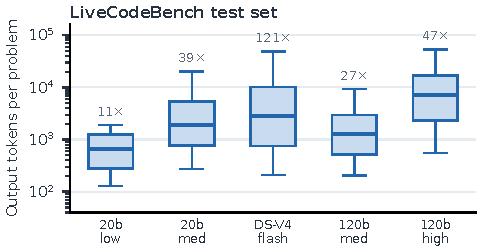
\includegraphics[width=.6\linewidth]{figures/length_spread.pdf}
\caption{\textbf{Output length varies by orders of magnitude within one model.} Per-problem output tokens by route on the LiveCodeBench test set (log scale). Boxes: interquartile range; whiskers: 5th--95th percentile; line: median; above each box: 90th/10th-percentile ratio.}
\label{fig:spread}
\end{figure}

Prefill routers predict correctness from a small encoder's prompt activations; the prefill router of Varshney et al.~\citep{prefill} explicitly prices outputs at median training length. We read output length from the same activations (\cref{fig:overview}). Cost prediction adds one linear readout per route to an existing prefill router, without another encoder pass.

This raises three questions, which organise the paper. When is per-query cost worth predicting? What does a prediction of it capture? And how cheaply can a router obtain it: with how many labels, for how many new models, and on how many new benchmarks?

We contribute:
(i) a measurement of what per-query cost knowledge is worth on nine pools, under one protocol at billed prices (29--60\% of spending at matched accuracy wherever reasoning lengths vary), and on the same problems with non-reasoning routes, where it is worth much less and is largely not legible from the prompt (\cref{sec:headroom});
(ii) prefill cost readouts that reduce spending by 28.8--34.8\% relative to median pricing on three large test sets and outperform mean-length, prompt-feature, text-embedding and ZeroRouter cost estimators (\cref{tab:fresh});
(iii) a mechanism: per-query length is mostly a problem-level property shared across routes; where it tracks difficulty, pricing from the success readouts alone is enough, and where it tracks the work a question requires, only a dedicated readout captures it (\cref{sec:mechanism}). The two failures we find have identifiable causes: too little headroom, or headroom that no estimator can read from the prompt (\cref{sec:when});
(iv) generalisation: the dedicated readout keeps most of its saving with few labels, when a new model is onboarded from a handful of examples, and when a router trained on other benchmarks is applied to a new one without labels, where the alternative estimators, including pricing from difficulty, do not (\cref{sec:general});
(v) controls showing the gain is the prefill representation: it holds for every small prefill we tried (0.6--8B, four families), and our linear readouts on fixed layers match the prefill router's full success pipeline.
As a side note, the same model's provider endpoints drift; the readouts can absorb this with one offset per endpoint, and we pin providers instead.

\paragraph{Related work.}
Learned routers pick one model per query from the prompt, trading predicted quality against price: RouteLLM learns a strong-versus-weak decision from preference data~\citep{routellm}, RouterBench standardizes the evaluation~\citep{routerbench}, and IRT-Router models query difficulty and model ability with item response theory~\citep{irtrouter}. Closest to us, the prefill router of Varshney et al.\ predicts each model's correctness from a small encoder's prompt activations~\citep{prefill}, and pre-generation activations are known to encode whether a model will fail~\citep{encodefailures}. These routers, like SWE-Router for agentic software engineering~\citep{swerouter}, price each model at a per-model constant; the prefill router uses the median training output length, which is our main reference. Fewer routers predict per-query cost: MixLLM regresses output length on query embeddings~\citep{mixllm}, CARROT uses embedding nearest neighbours or a fine-tuned RoBERTa~\citep{carrot}, GraphRouter predicts cost on a query--model graph~\citep{graphrouter}, Route-To-Reason predicts reasoning-model length from text embeddings~\citep{routetoreason}, and ZeroRouter prices queries by item-response difficulty bins~\citep{zerorouter}. We compare against the embedding-based and ZeroRouter estimators directly, with every estimator given the same success predictions.

Cascades instead call models in sequence and stop when an answer is accepted: FrugalGPT learns a scorer that decides whether to escalate~\citep{frugalgpt}, AutoMix uses self-verification~\citep{automix}, and Dekoninck et al.\ unify routing and cascading~\citep{cascaderouting}. A cascade pays for the cheap attempt on every query; we route once, before generation. Activation-based length prediction also supports serving and scheduling of a single model~\citep{alps,egtp}; we predict the length of other models from one shared prefill. Hosted open-weight models vary across providers in accuracy, length and price~\citep{samemodel,gateways,modelequality}, and FACET selects among providers of a fixed model per task from measured outcomes~\citep{facet}.

\begin{figure}[t]
\centering
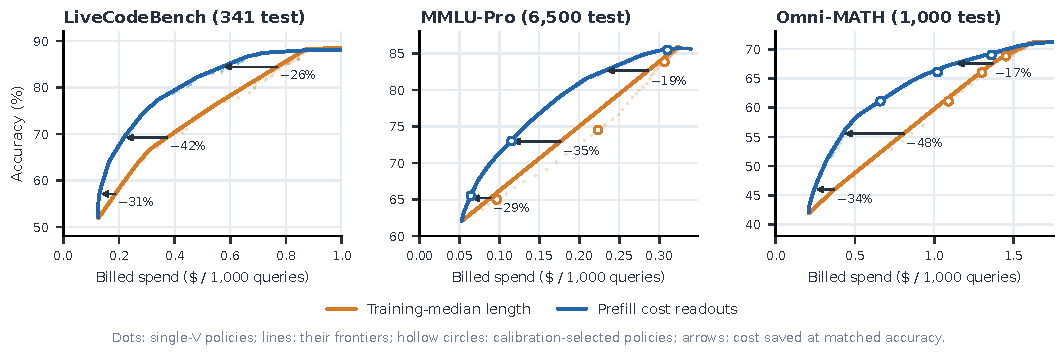
\includegraphics[width=\linewidth]{figures/shared_prefill_overview.pdf}
\caption{\textbf{Cost--accuracy frontiers at billed prices.} Prefill cost readouts (blue) versus training-median length (orange), with the same success predictions and the same encoder pass. Dots: the deterministic policy at each $V$; lines: their frontiers; hollow circles: policies selected on calibration for fixed accuracy targets. Arrows run from the median rule's frontier to ours at matched accuracy and give the cost saved; averaged over the shared accuracy band the saving is 34\% on LiveCodeBench, 29\% on MMLU-Pro and 35\% on Omni-MATH.}
\label{fig:overview}
\end{figure}

\section{Cost Prediction and Routing}
For query $x$ and route $m$ (a model at a fixed reasoning effort, served by an endpoint), let $p_m(x)$ be the probability of a correct answer and $c_m(x)$ the expected generation cost. One route is chosen before generation,
\begin{equation}
m^*(x;V)=\arg\max_m\{V\hat p_m(x)-\hat c_m(x)\},
\label{eq:route}
\end{equation}
where $V$ is the value of a correct answer; sweeping $V$ trades accuracy for cost. Every query is answered once, with no verifier or fallback.

\paragraph{Readouts.}
We concatenate mean and last-token activations from eight layers of a frozen Qwen3-4B (Instruct-2507; Thinking-2507 on Omni), standardized on training data. Success readouts are L2-regularized logistic regressions with held-out Platt calibration; cost readouts are ridge regressions of log mean output length, regularized by training-only cross-validation. Predicted length is exponentiated with residual smearing and matched to the route's training mean, then priced: $\hat c_m(x)=r_m^{\rm in}n^{\rm in}_m(x)+r_m^{\rm out}\hat\ell_m(x)$.

\section{Experimental Protocol}
The routes are gpt-oss-20b at low and medium effort, deepseek-v4-flash, and gpt-oss-120b at medium and high effort, called through OpenRouter, with deepseek-v4-flash pinned to one provider (StreamLake) throughout, because its output length depends on the serving provider (see Endpoints). LiveCodeBench~\citep{lcb} has 892 problems split by date into 441 training, 110 calibration and 341 test problems. Omni-MATH~\citep{omni} and MMLU-Pro~\citep{mmlupro} have 275/75 and 550/150 training/calibration problems and 1,000 and 6,500 disjoint test problems. Training problems have 2--16 draws per route; Omni-MATH and MMLU-Pro test problems have one. \Cref{tab:routes} gives each route's accuracy and cost.

\paragraph{Prices.}
Realized cost is the cost billed for each call (on LCB, realized tokens at the billed rates). Predictions are priced at each model's effective billed rate, fitted on the test calls (USD per million output tokens: 0.13 for gpt-oss-20b, 0.08 for pinned deepseek-v4-flash, 0.26 for gpt-oss-120b). These differ from the list prices by up to 2.3$\times$.

\paragraph{Evaluation.}
All estimators are fitted on training problems only and evaluated on the test sets, with the same success predictions. Each $V$ on a dense grid gives a deterministic policy and an observed (cost, accuracy) point. Comparing two cost estimators $a,b$, we interpolate each one's cost at 12 accuracies spanning the interior 90\% of the range both reach and report $1-\exp(\overline{\log C_a/C_b})$, the cost saved by $a$ at matched accuracy. Intervals are percentile intervals from paired problem bootstraps (300 resamples), keeping each problem's routes together. As an upper bound, an oracle arm prices each problem at its realized cost; its saving over median pricing is the headroom, and our share of it the capture. To check that an operating point can be chosen in advance, we also select the cheapest $V$ reaching each accuracy target on calibration and apply it once.

\begin{table}[t]
\centering
\footnotesize
\setlength{\tabcolsep}{2.5pt}
\resizebox{\linewidth}{!}{%
\begin{tabular}{lrrr}
\toprule
Cost saved by ours vs. & LCB ($n$=341) & Omni-MATH ($n$=1,000) & MMLU-Pro ($n$=6,500) \\
\midrule
Training-median length & 33.7 [24.1, 39.9] & 34.8 [27.9, 39.8] & 28.8 [26.0, 31.8] \\
Training-mean length & 29.6 [23.6, 34.5] & 35.8 [28.9, 40.5] & 28.6 [25.9, 31.7] \\
Prompt-feature GBM & 26.3 [16.3, 32.9] & 26.5 [18.9, 31.9] & 25.2 [21.0, 28.7] \\
MixLLM-style embeddings & 18.2 [11.2, 25.2] & 26.7 [20.0, 32.5] & 19.2 [15.3, 22.5] \\
ZeroRouter (reimplemented) & 21.1 [13.2, 26.8] & 14.4 [8.4, 20.6] & 29.0 [25.5, 32.0] \\
\midrule
\emph{Headroom: oracle vs.\ median} & 45.3 [36.6, 50.4] & 55.5 [50.4, 58.8] & 59.5 [57.8, 61.2] \\
\bottomrule
\end{tabular}}
\caption{\textbf{Cost saved at matched accuracy, billed costs.} Cost saved (\%) by our prefill cost readouts relative to each estimator, with 95\% paired bootstrap intervals; same success predictions for every arm except ZeroRouter, which uses its own; all intervals exclude zero. Last row: cost saved over median pricing by perfect per-query cost knowledge (each problem priced at its realized output), with the same success predictions; our readouts capture 74\%, 63\% and 49\% of it. Test sets as in \cref{fig:overview}. Prompt-feature GBM: gradient boosting on prompt statistics, as in latency-aware routing~\citep{latencyrouting}. MixLLM-style: jina-embeddings 137M with the MixLLM ensemble head (LCB, code-aware variant). ZeroRouter: item-response latent fitted on the five routes, 4B features, its own success model and bin pricing, configuration chosen on calibration.}
\label{tab:fresh}
\end{table}

\begin{table}[t]
\centering
\footnotesize
\setlength{\tabcolsep}{3pt}
\resizebox{\linewidth}{!}{%
\begin{tabular}{lrrrrrr}
\toprule
 & \multicolumn{2}{c}{LCB} & \multicolumn{2}{c}{Omni-MATH} & \multicolumn{2}{c}{MMLU-Pro} \\
\cmidrule(lr){2-3}\cmidrule(lr){4-5}\cmidrule(lr){6-7}
Route & Acc. & Cost & Acc. & Cost & Acc. & Cost \\
\midrule
gpt-oss-20b, low & 51.8 & 0.13 & 41.9 & 0.21 & 62.1 & 0.05 \\
gpt-oss-20b, medium & 68.2 & 0.65 & 57.5 & 1.20 & 69.4 & 0.18 \\
deepseek-v4-flash & 89.3 & 0.90 & 71.3 & 1.66 & 86.2 & 0.33 \\
gpt-oss-120b, medium & 82.1 & 0.64 & 60.3 & 1.12 & 77.2 & 0.23 \\
gpt-oss-120b, high & 89.5 & 3.73 & 66.6 & 4.57 & 79.3 & 0.90 \\
\bottomrule
\end{tabular}}
\caption{\textbf{Routes on the test sets.} Accuracy (\%) and mean billed cost per call (USD per 1,000 calls). No route dominates on every query: costs differ 17--29$\times$ across routes, and accuracy is not monotone in price.}
\label{tab:routes}
\end{table}


\section{Results}
\paragraph{Cost readouts beat every estimator.}
At matched accuracy, prefill cost readouts spend 33.7\% less than median-length pricing on LCB, 34.8\% less on Omni-MATH and 28.8\% less on MMLU-Pro (\cref{tab:fresh}). That is 74\%, 63\% and 49\% of the headroom, the saving perfect per-query cost knowledge would bring (45--60\%). Every external estimator loses with intervals excluding zero: mean length by 29--36 points, a prompt-feature model by 25--27, MixLLM-style embeddings by 18--27 and a full ZeroRouter reimplementation by 14--29. Choosing $V$ in advance costs little: on Omni-MATH and MMLU-Pro, policies selected on calibration spend 0--4\% more than our own test frontier at the accuracy they reach (hollow circles in \cref{fig:overview}).


\paragraph{Endpoints.}
The same model served by different providers behaves like the model plus an offset: pinning deepseek-v4-flash to each of three providers, they agree on correctness for 90--96\% of problems and their output lengths correlate at .83--.95, but one writes about half as many tokens as another. Reusing the readouts with one multiplicative length offset per endpoint, estimated from 50 calls, removes the resulting cost bias on average, though a single estimate is noisy. A few dozen calls per provider also identify the cheapest one, and pinning it beats routing over providers; we therefore pin deepseek-v4-flash throughout, which also makes its length more predictable and raises our saving on every large set.

\paragraph{Other pools.}
On the remaining six pools (\cref{tab:pools}) our readouts save 15.7\% [11.7, 20.6] on AIME, 15.1\% [5.0, 26.9] on APPS, 27.6\% [11.0, 38.2] on SuperGPQA and 26.5\% [16.4, 34.3] on BIG-Bench Extra Hard relative to median pricing; \cref{sec:when} treats BigCodeBench and CodeContests, where no estimator saves significantly.

\section{How much is per-query cost worth?}\label{sec:headroom}
A cost estimator can be no better than knowing each query's realized cost. We therefore measure, on every pool, the \emph{headroom}: the cost saved at matched accuracy when each test problem is priced at its realized cost instead of the training median, with the same success predictions. \Cref{tab:pools} reports it with our saving and the share of it we capture, on nine pools under one protocol (five routes, deepseek-v4-flash pinned, billed rates, test splits).

\begin{table}[t]
\centering
\footnotesize
\setlength{\tabcolsep}{4pt}
\begin{tabular}{llrrrrr}
\toprule
Pool & Domain & Test $n$ & Headroom & Ours vs.\ median & Capture & Ours vs.\ cost-from-success \\
\midrule
LiveCodeBench & code & 341 & 45.3 & 33.7 [24.1, 39.9] & .74 & $-0.8$ \\
Omni-MATH & math & 1,000 & 55.5 & 34.8 [27.9, 39.8] & .63 & $-0.1$ \\
MMLU-Pro & knowledge & 6,500 & 59.5 & 28.8 [26.0, 31.8] & .49 & \textbf{24.1} \\
AIME 1983--2024 & math & 281 & 29.3 & 15.7 [11.7, 20.6] & .54 & 2.0 \\
APPS & code & 377 & 32.1 & 15.1 [5.0, 26.9] & .47 & $-3.7$ \\
BigCodeBench & code & 421 & 12.6 & 6.3 [$-$1.6, 11.8] & .50 & 3.2 \\
CodeContests & code & 266 & 34.5 & 6.3 [$-$0.2, 17.0] & .18 & 0.7 \\
\midrule
SuperGPQA & knowledge & 300 & 57.0 & 27.6 [11.0, 38.2] & .48 & \textbf{9.0} \\
BIG-Bench Extra Hard & reasoning & 298 & 41.8 & 26.5 [16.4, 34.3] & .63 & \textbf{26.6} \\
\bottomrule
\end{tabular}
\caption{\textbf{Headroom and capture on every pool.} Cost saved (\%) at matched accuracy relative to median-length pricing: by perfect per-query cost knowledge (headroom) and by our readouts (95\% paired bootstrap intervals); capture is their ratio. Last column: cost saved by our dedicated cost readout relative to our ablation that prices from the success readouts alone; bold: interval excludes zero. Billed costs, deepseek-v4-flash pinned, same success predictions in every column.}
\label{tab:pools}
\end{table}

\paragraph{Headroom is large wherever reasoning lengths vary.}
On seven of nine pools perfect per-query cost knowledge would save 29--60\%, and our readouts capture about half of it or more. The exceptions are informative. BigCodeBench has little to capture (12.6\%), and CodeContests has headroom that our readouts do not reach (capture .18); \cref{sec:when} shows that no estimator reaches it.

\paragraph{Length, not only price gaps, makes it pay.}
To separate the two sources of headroom, we rescale every route's billed price toward or away from the cheapest route's while keeping realized lengths fixed. With all routes at the same per-token price, our readouts still save 13.3\% (LCB), 14.3\% (Omni-MATH) and 36.3\% (MMLU-Pro) relative to median pricing: per-query length alone is worth that much. On LCB and Omni-MATH the saving grows with the price gap and saturates near the billed gap (3.1$\times$); on MMLU-Pro it is largest at flat prices (36.3\%, against 28.8\% at billed prices), because there length differs between questions rather than between routes.

\paragraph{Choosing effort and choosing the model are both needed.}
Restricting the pool removes most of the saving. With only gpt-oss-20b's two efforts, ours saves 21.2\% (LCB), 21.8\% (Omni-MATH) and 7.9\% (MMLU-Pro); with only gpt-oss-120b's, $-$1.8\%, 12.6\% and 8.6\%; with one effort per model, 12.8\% and 17.8\% on LCB and Omni-MATH; with all five routes, 33.7\%, 34.8\% and 28.8\%.

\paragraph{Reasoning makes per-query cost worth predicting.}
To test whether this is a property of reasoning models, we collected five non-reasoning routes on the same problems: deepseek-v4-flash with thinking disabled (same provider and sampling), Llama-3.1-8B, Qwen3-30B-A3B-Instruct, Llama-3.3-70B and Qwen3-235B-A22B-Instruct, each pinned to one provider, one draw per problem, with output capped at 16k tokens. Readouts are fitted exactly as for the reasoning routes. \Cref{tab:nonreason} compares the two pools on the common test problems. Headroom is 1.4--2.3$\times$ larger with reasoning routes, and our saving is 1.7$\times$ (LCB) to about 24$\times$ (MMLU-Pro) larger; on MMLU-Pro the non-reasoning saving is not distinguishable from zero. Non-reasoning lengths do vary (s.d.\ of log length .53--1.73 per route), but much of that variation is degenerate output that the prompt does not predict: Llama-3.1-8B repeats until the cap on a minority of problems (its mean output is 4--6$\times$ its median; log-length $R^2$ below zero on every set), and Qwen3-30B-A3B-Instruct's LCB lengths span 142$\times$ between its 10th- and 90th-percentile problems ($R^2$ .27). Where non-reasoning routes do leave headroom, it is mostly this kind. Adding the non-reasoning routes to the reasoning pool lowers our saving (17.7\% on Omni-MATH, 13.0\% on MMLU-Pro, 24.9\% on LCB). The same model with thinking on and off shows the trade directly: deepseek-v4-flash with thinking gains 2.8 (MMLU-Pro), 14.6 (Omni-MATH) and 22.1 (LCB) points of accuracy for 13$\times$, 11$\times$ and 33$\times$ the output, and the problems that are long with thinking are long without it (correlation of log length .66--.76).

\begin{table}[t]
\centering
\footnotesize
\setlength{\tabcolsep}{4pt}
\begin{tabular}{lrrrrrr}
\toprule
 & \multicolumn{2}{c}{Headroom} & \multicolumn{2}{c}{Ours vs.\ median} & \multicolumn{2}{c}{Capture} \\
\cmidrule(lr){2-3}\cmidrule(lr){4-5}\cmidrule(lr){6-7}
Test set & reasoning & non-reas. & reasoning & non-reas. & reasoning & non-reas. \\
\midrule
LiveCodeBench (341) & 45.3 & 28.9 & 33.7 & 19.7 [7.7, 29.2] & .74 & .68 \\
Omni-MATH (1,000) & 55.5 & 40.7 & 34.8 & 7.2 [3.7, 10.8] & .63 & .18 \\
MMLU-Pro (2,000) & 60.5 & 26.0 & 30.6 & 1.3 [$-$2.4, 5.3] & .51 & .05 \\
\bottomrule
\end{tabular}
\caption{\textbf{Reasoning versus non-reasoning routes on the same problems.} Headroom (perfect per-query cost knowledge vs.\ median pricing), our saving relative to median pricing (95\% paired bootstrap intervals) and capture, for the five reasoning routes and for five non-reasoning routes, on the test problems where every route of both pools has a valid answer (MMLU-Pro: a 2,000-problem subset of the test set). Billed costs; readouts fitted on the same training problems with the same recipes. Qwen3-235B-A22B-Instruct has training answers for 241 of 275 Omni-MATH and 485 of 550 MMLU-Pro problems (rate limits).}
\label{tab:nonreason}
\end{table}

\section{What the cost readout captures}\label{sec:mechanism}
\paragraph{Length is mostly a property of the problem.}
The prefill explains much of each route's log output length on held-out problems (5-fold cross-validated $R^2$: .73--.77 on LCB, .74--.83 on Omni-MATH, .52--.66 on MMLU-Pro, .43--.57 on AIME). On LCB, Omni-MATH and AIME most of this is shared with difficulty: a problem's empirical solve rate across routes alone reaches $R^2$ .48--.65, and the prefill misses at most .07 of what difficulty explains (.10--.22 on AIME). Within a problem, failed and solved draws are about equally long ($\times$0.83--1.16), with one exception: deepseek-v4-flash writes 2.5$\times$ (Omni-MATH) and 1.9$\times$ (AIME) longer when it fails on hard math.

\paragraph{The shared level carries most of the value.}
A problem's lengths across routes can be split into a shared level (their mean) and route-specific differences. On LCB, an oracle that knows only each problem's level captures 87\% of the headroom, about as much as one that knows only the differences. The prefill reads the level far better ($R^2$ .75) than the differences (.41); pricing with the predicted level alone keeps 33.2 of the full readout's 36.4 points (list prices).

\paragraph{Success and cost are read from the same layers.}
Refitting both readouts on each stored layer separately, success AUC and length $R^2$ peak in the same late layers at the last token (layers 22--36 of 36), and one such layer matches the full concatenation (LCB AUC .86--.87, $R^2$ .73--.75, saving 33--34\%; Omni-MATH .83--.84, .71--.72, 35--37\%; MMLU-Pro .72, .48--.50, 27--29\%). The two readouts are close to one signal where length tracks difficulty: the mean success logit correlates with predicted log length at $-$.90 to $-$.97 per layer on LCB and $-$.71 to $-$.84 on Omni-MATH, but only $-$.36 to $-$.58 on MMLU-Pro.

\paragraph{Where length tracks work rather than difficulty.}
On MMLU-Pro, difficulty explains log length only in part (test $R^2$ .18--.37), subject labels about as much (.17--.25), and the two together .34--.44, against .41--.66 for the prefill. Engineering and law questions are both long (6.4k and 4.1k output tokens on average) and hard. Pricing from difficulty and subject together saves 30.3\%, against 43.9\% for the prefill (headroom 64.1\%, list prices): the prefill reads how much work a question requires, beyond its difficulty and topic.

\paragraph{Two further heterogeneous pools.}
We chose SuperGPQA~\citep{supergpqa} and BIG-Bench Extra Hard~\citep{bbeh} as further pools because, on a cheap screen (one gpt-oss-20b-low draw per problem), length predicted directly from the prefill beat length predicted from a success readout by a margin as large as MMLU-Pro's ($R^2$ gap .61 and .40, against .66 on MMLU-Pro and .10 on Omni-MATH). On their full pools the dedicated readout again beats pricing from success: by 26.6\% [17.8, 34.9] on BIG-Bench Extra Hard, where pricing from success saves nothing over the median, and by 9.0\% [0.1, 15.4] on SuperGPQA (\cref{tab:pools}). On BIG-Bench Extra Hard, text-only estimators read length as well as the prefill: MixLLM-style embeddings save 28.0\% relative to median pricing (ours $-$2.2 [$-$5.7, 1.8] relative to it). Its 23 tasks have very different formats, and the task is visible in the text. On SuperGPQA they do not (ours saves 15.2\% [$-$1.4, 25.4] relative to MixLLM-style and 18.8\% [5.6, 29.6] relative to prompt features).

\paragraph{How many length labels are needed.}
Given success readouts, where length tracks difficulty a cost readout needs few length labels (\cref{fig:labels}). Pricing from the success logits reaches 27.8\% (LCB) and 31.5\% (Omni-MATH) with 20 labelled training problems, against 24.7\% and 22.8\% for a dedicated readout. On MMLU-Pro it plateaus at about 6\%, while the dedicated readout climbs to 22.6\% at 100 problems and 28.8\% at all 550. One draw per training problem instead of all draws gives up 1--3 points.
\begin{figure}[t]
\centering
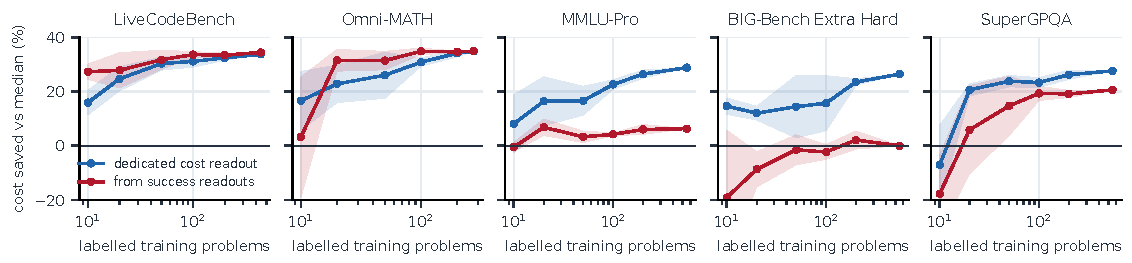
\includegraphics[width=\linewidth]{figures/label_efficiency.pdf}
\caption{\textbf{Length labels needed.} Cost saved relative to median pricing when the cost readout is fitted on $n$ labelled training problems: a dedicated readout on the prefill (blue) versus pricing from the success readouts (red), which needs length labels only to map success logits to length. Mean over five random subsets; bands $\pm$1 s.d. Where length tracks difficulty (LiveCodeBench, Omni-MATH), pricing from success is as good from 20 problems on; where it tracks the work a question requires (MMLU-Pro, BIG-Bench Extra Hard), it stays near zero at every $n$.}
\label{fig:labels}
\end{figure}

\paragraph{What changes in the routing.}
At matched accuracy in the middle of the band, 31--66\% of problems change route relative to median pricing. The dominant changes are between gpt-oss-20b-low and deepseek-v4-flash: problems predicted to be short move to the more accurate deepseek-v4-flash (19--38\% of problems), and problems predicted to be long move to the cheap route (9--18\%).

\section{How cheaply can a router get it?}\label{sec:general}
Where length tracks difficulty, pricing from the success readouts ties the dedicated cost readout when both are fitted on a benchmark's full training set (\cref{tab:pools}). A deployed router rarely has that: it has few labels, it adds models, and it meets benchmarks it was not trained on. We test the cost estimators in all three settings, with every estimator given the same success predictions unless stated, and the same protocol as before.

\paragraph{Few labels.}
\Cref{tab:labels} refits every cost estimator on 20 randomly chosen training problems (five subsets). Our readout keeps 57--75\% of its full-data saving on four of five pools (LCB 24.7\%, Omni-MATH 22.8\%, MMLU-Pro 16.4\%, SuperGPQA 20.6\%), while the external estimators save less than 11\% on every pool. Their deficit narrows with data but stays large on most pools: at 100 problems ours saves 22.6\% on MMLU-Pro against at most 10.6\% for any external estimator, with every paired interval excluding zero. The exception is BIG-Bench Extra Hard, where the task format is visible in the text: the text estimators reach 19--22\% at 100 problems and tie ours at full data. Pricing from the success readouts is the strongest arm on LCB and Omni-MATH from 20 problems on, as in \cref{fig:labels}, and far behind ours on the two heterogeneous pools.

\begin{table}[t]
\centering
\footnotesize
\setlength{\tabcolsep}{4pt}
\begin{tabular}{lrrrrr}
\toprule
Cost estimator, 20 training problems & LCB & Omni-MATH & MMLU-Pro & SuperGPQA & BBEH \\
\midrule
Ours (prefill readout) & \textbf{24.7} & 22.8 & \textbf{16.4} & \textbf{20.6} & 10.6 \\
Cost from success (our ablation) & 27.8 & 31.5 & 6.8 & 5.9 & $-$15.0 \\
Prompt-feature GBM & $-$7.7 & 0.1 & 2.8 & 2.3 & 2.3 \\
MixLLM-style embeddings & $-$1.8 & 7.0 & 2.5 & 3.4 & $-$5.8 \\
CARROT-style $k$NN & 0.1 & 6.0 & 10.7 & 7.4 & $-$1.4 \\
ZeroRouter pricing & 7.6 & 9.3 & 3.5 & $-$9.2 & $-$3.6 \\
\midrule
\emph{Ours, all training problems (refit)} & 33.7 & 34.8 & 28.8 & 27.6 & 26.1 \\
\bottomrule
\end{tabular}
\caption{\textbf{Few labels.} Cost saved (\%) relative to median pricing (from the full training set) when each cost estimator is fitted on 20 random training problems; mean of five subsets; every arm routes with the same success readouts. ZeroRouter pricing: its item-response latent fitted on the 20 problems, read from the prefill, with its bin lookup; $k$NN neighbours and ZeroRouter's dimension and bin count chosen on the calibration split. Bold: ours exceeds every external estimator with paired intervals excluding zero (LCB from $n$=20, SuperGPQA from $n$=50, MMLU-Pro from $n$=100).}
\label{tab:labels}
\end{table}

\paragraph{New models.}
To add a model, a router needs its success and cost readouts. We hold out one model at a time from the pool (both efforts of gpt-oss-20b, both efforts of gpt-oss-120b, or deepseek-v4-flash, so that no sibling effort of the new model remains) and fit its readouts from $k$ labelled problems while every other route keeps its full readouts. Our onboarding fits two parameters per readout: an offset to the other routes' predicted log length, and a logistic map from their mean success logit. ZeroRouter's onboarding, its main use case, fits the new model's ability on the same $k$ anchors in an item-response latent fitted on the remaining routes and fills its per-bin length table from them~\citep{zerorouter}; a CARROT-style arm averages the $k$ anchors' outcomes and lengths over nearest neighbours. \Cref{tab:onboard} reports the mean over the three held-out models. From 10 examples our router saves 13.5--25.6\%, against 5.8--22.4\% for ZeroRouter's onboarding, and leads it by 10.1 [1.4, 23.7] points on MMLU-Pro and 14.6 [3.0, 26.0] on SuperGPQA; at $k$=50 it also leads on LCB (9.3 [3.0, 17.0]). On Omni-MATH and BIG-Bench Extra Hard the two are within noise. The gain concentrates on deepseek-v4-flash, the one model whose family is not otherwise in the pool, and whose absence makes the router spend more than median pricing on four of five pools: onboarding it from 10 problems recovers 10--35 points more than ZeroRouter's onboarding does. ZeroRouter's Fisher-information anchors help both methods about equally; with the same anchors ours ties on LCB and Omni-MATH and leads by 6--16 points on the other three pools at $k$=10.
\todo{New routed families (Qwen3-32B, GLM-4.7-flash, Nemotron-3-super) on all three main sets are being collected (NEW\_PATH 4.A.76): whole-family onboarding beyond one cross-family model; add a row block or replace the held-out set.}

\begin{table}[t]
\centering
\footnotesize
\setlength{\tabcolsep}{4pt}
\begin{tabular}{lrrrrr}
\toprule
 & LCB & Omni-MATH & MMLU-Pro & SuperGPQA & BBEH \\
\midrule
Ours, $k$=10 & 24.6 & 25.6 & 22.6 & 20.4 & 13.5 \\
ZeroRouter onboarding, $k$=10 & 13.6 & 22.4 & 12.6 & 5.8 & 6.0 \\
CARROT-style $k$NN, $k$=10 & 13.3 & 15.3 & 8.5 & 7.4 & 11.9 \\
Median length + base rate, $k$=10 & $-$7.1 & 10.6 & 2.9 & 3.5 & 5.8 \\
\midrule
Ours $-$ ZeroRouter, $k$=10 & 10.9 [$-$2.0, 24.1] & 3.2 [$-$12.3, 27.9] & 10.1 [1.4, 23.7] & 14.6 [3.0, 26.0] & 7.5 [$-$2.2, 17.9] \\
Ours $-$ ZeroRouter, $k$=50 & 9.3 [3.0, 17.0] & $-$0.2 [$-$7.3, 6.0] & 9.6 [2.2, 14.8] & 12.8 [5.8, 23.0] & 4.2 [$-$1.6, 16.6] \\
\midrule
\emph{All routes on full readouts} & 33.7 & 34.8 & 28.8 & 27.6 & 26.5 \\
\bottomrule
\end{tabular}
\caption{\textbf{Onboarding a new model from $k$ examples.} Cost saved (\%) relative to the full pool at median pricing, mean over three held-out models (gpt-oss-20b with both efforts, gpt-oss-120b with both efforts, deepseek-v4-flash) and 20 random draws of the $k$ anchors (the same anchors in every arm); every other route keeps its full readouts. Differences in points with 95\% paired bootstrap intervals over test problems. ZeroRouter's dimension and bin count and the $k$NN neighbour count are chosen on calibration.}
\label{tab:onboard}
\end{table}

\paragraph{New benchmarks.}
Finally, we move a whole router to a benchmark it has not seen: both readouts are trained on the other pools of the same domain (code, or math and knowledge), with every choice (regularisation, Platt calibration, neighbour counts, latent dimension, bin count) made on those pools' calibration splits, so no label of the target is used. \Cref{tab:transfer} compares it with the router trained on the target itself. On LCB, MMLU-Pro and AIME the transferred router keeps 90--95\% of its in-domain saving (32.1\%, 27.3\% and 14.2\%), and on APPS it exceeds it. The prefill router's rule, the same transferred success readouts with median pricing, saves at most 2\% on any of these, so the transferred cost readout carries the result, even though transferred success predictions are weaker (LCB AUC .65 against .83). Ours leads every external estimator transferred the same way, by 7--24 points on these four pools. Transfer is weaker on the two heterogeneous pools and on Omni-MATH (7.3--19.0\%). Combining both sources of labels is better than either: with ten labelled target problems added to the source data, the cost readout saves 27.8\% on MMLU-Pro and 13.1\% on AIME (with the target's success readouts), against 8.1\% and 4.4\% from the ten problems alone, and 21.7\% against 10.6\% on BIG-Bench Extra Hard with twenty. Pricing from the success readouts does not transfer: trained on the other pools it saves $-$6.2\% on LCB, $-$19.9\% on SuperGPQA and $-$16.9\% on BIG-Bench Extra Hard with the target's own success readouts, where the dedicated readout saves 30.2\%, 17.5\% and 11.3\% under the same conditions.

\begin{table}[t]
\centering
\footnotesize
\setlength{\tabcolsep}{4pt}
\begin{tabular}{lrrrr}
\toprule
 & Ours, & Ours, & Prefill-router rule, & Best external, \\
Target & in-domain & transferred & transferred & transferred \\
\midrule
LiveCodeBench & 33.7 & 32.1 & 2.0 & 7.8 (MixLLM) \\
APPS & 12.8 & 21.7 & $-$0.7 & 11.0 (MixLLM) \\
MMLU-Pro & 28.8 & 27.3 & $-$1.4 & 17.2 ($k$NN) \\
AIME & 15.7 & 14.2 & $-$1.6 & 6.8 ($k$NN) \\
SuperGPQA & 27.6 & 19.0 & $-$23.2 & 6.0 (MixLLM) \\
BIG-Bench Extra Hard & 26.1 & 7.3 & $-$21.0 & $-$6.2 (MixLLM) \\
Omni-MATH (500-problem pool) & 18.2 & 8.1 & $-$20.0 & 4.3 (MixLLM) \\
\bottomrule
\end{tabular}
\caption{\textbf{A router moved to a new benchmark.} Cost saved (\%) relative to the target's own median rule, at matched accuracy on its test set. Transferred: success and cost readouts trained on the other pools of the same domain (coding: LCB, APPS, BigCodeBench, CodeContests; math and knowledge: Omni-MATH, MMLU-Pro, AIME, SuperGPQA, BIG-Bench Extra Hard), with every choice made on their calibration splits. Prefill-router rule: the transferred success readouts with median pricing. External estimators transferred the same way, each with its own success model (MixLLM-style: logistic readout on the text embedding; $k$NN; ZeroRouter: its latent and bins). Ours exceeds every other arm with paired intervals excluding zero on LCB, MMLU-Pro, AIME and BIG-Bench Extra Hard. Omni-MATH uses its 500-problem pool (test 150), whose prefill matches the other pools'. BigCodeBench and CodeContests, where no in-domain estimator saves significantly, are omitted: there the transferred success readouts are badly miscalibrated (BigCodeBench log loss 1.17 against .67 in-domain) and the apparent gains are not robust.}
\label{tab:transfer}
\end{table}

\paragraph{Why the cost readout transfers.}
Training one readout on the target together with the other pools matches the target-only readout within about 3 points on every pool, so a single readout can serve all of them. Part of what transfers is shared structure: 24--40\% of each route's variance in log length lies between benchmarks, and the routes agree on which benchmarks are long (mean correlation of benchmark means across routes .84). Length $R^2$ under transfer is close to in-domain on LCB, APPS, AIME, Omni-MATH and SuperGPQA but falls sharply on MMLU-Pro (.02--.46 against .29--.63), where routing transfers fully nonetheless: routing needs the ordering of problems within a route and the contrast between routes, not calibrated absolute lengths.

\section{When it works and when it does not}\label{sec:when}
Per-query cost pays under two conditions: (a) output length varies within a route by more than prices differ between routes, which creates headroom, and (b) that variation can be read from the prompt, which lets an estimator capture it. Each of our two failures violates one condition, and neither is specific to our estimator (\cref{fig:capture}).

\paragraph{Little headroom: BigCodeBench.}
BigCodeBench tasks are library-usage functions with short, similar solutions; perfect cost knowledge saves only 12.6\% [4.1, 19.0]. No estimator's saving relative to median pricing has an interval excluding zero: ours 6.3 [$-$1.6, 11.8], ZeroRouter 8.8 [$-$12.5, 19.6], MixLLM-style 2.8, cost-from-success 3.1, prompt features 0.2. Here length is the least tied to difficulty of any pool (the prefill-only share of length variance is largest on BigCodeBench), but there is little to gain from reading it.

\paragraph{Illegible headroom: CodeContests.}
CodeContests has as much headroom as APPS (34.5\% [29.0, 42.0]), but no estimator captures more than about a quarter of it: ZeroRouter saves 9.3\% [1.1, 20.0], difficulty bins 5.6\% [1.2, 14.6], ours 6.3\% [$-$0.2, 17.0], and the rest are within noise of zero or below it. Length again tracks difficulty, but difficulty itself is hard to read from these prompts: the prefill misses .11--.18 of the length $R^2$ that empirical difficulty explains, against at most .07 on LCB and Omni-MATH.

\begin{figure}[t]
\centering
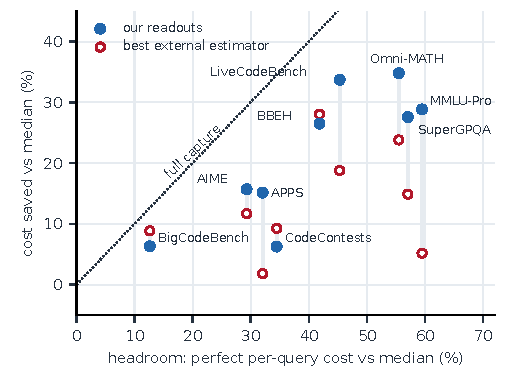
\includegraphics[width=.55\linewidth]{figures/capture_map.pdf}
\caption{\textbf{Headroom and capture.} Per pool: the saving of perfect per-query cost knowledge over median pricing (x) against the saving of our readouts (filled) and of the best external estimator on that pool (hollow; mean length, prompt features, MixLLM-style embeddings or ZeroRouter). Triangles: our readouts with five non-reasoning routes on the same LiveCodeBench, Omni-MATH and MMLU-Pro test problems (\cref{tab:nonreason}). Billed costs, test splits, deepseek-v4-flash pinned. Where headroom is large and length is legible, the readouts capture half or more of it; on BigCodeBench there is little to capture, on CodeContests no estimator captures it, and non-reasoning routes leave less headroom, which on Omni-MATH and MMLU-Pro is almost all illegible.}
\label{fig:capture}
\end{figure}
\paragraph{Non-reasoning routes.}
Non-reasoning routes combine both failures (\cref{tab:nonreason}): less headroom, and on Omni-MATH and MMLU-Pro a capture of .18 and .05, because much of their length variation is degenerate output. On LCB the readouts capture .68 of a smaller headroom.
\todo{RouterBench chat (little length variation) as a further low-headroom point, if rerun on this protocol.}

\section{Software engineering}\label{sec:swe}
Software engineering is where per-query cost is hardest to use. We study it in two regimes, one-shot patch generation and agents.

\paragraph{One-shot patches.}
On 500 SWE-Smith instances~\citep{swesmith}, each of the five routes writes one patch per draw, labelled by executing the repository's tests. Pass rates are low and close together (23--36\%), and the success readouts are nearly flat. Per-query cost knowledge is worth 14.2\% [$-$2.1, 29.6] on the 150 test instances, and our readouts save 7.5\% [$-$5.5, 20.0]: with little to choose between routes on correctness, knowing their costs helps little, even though length is predictable for the gpt-oss routes (log-length $R^2$ .49--.72; .20 for deepseek-v4-flash).

\paragraph{Agents: cost is real, varies by task and is stable.}
Public SWE-rebench trajectories~\citep{swerebench} give 111 tasks run five times by each of 13 models in one scaffold. Across models, agentic cost is dominated by the model: of the variance of log cost, 74\% is between models, 15\% between tasks, 6\% their interaction and 4\% run to run. Within a model, however, per-task cost spans 2.7--9.0$\times$ between the 10th and 90th percentile, and it is stable across runs (intraclass correlation .69--.92). Whether knowing it pays depends on the price gaps between the routed models, as in \cref{sec:when}: among all 13 models, whose prices per run span about 190$\times$, per-task cost knowledge is worth 8.5\% [$-$5.0, 17.8] (one-shot routing, success and cost from three runs, scored on the other two); among the seven open-weight models, whose prices span about 10$\times$, it is worth 25.7\% [6.3, 40.6], as much as on the reasoning pools.

\paragraph{Agents: cost is only partly legible before the run.}
From the issue text alone, the prefill's cost readout reaches out-of-fold $R^2$ of about zero on the 111 SWE-rebench tasks, too few to fit it. On 3,387 tasks with about 20 SWE-agent runs each (one model, Llama-3.1-70B; cost proxied by cumulative context and output length), the per-task mean cost is reliable (split-half reliability .91) and the issue text predicts it at $R^2$ .29, still rising with data (.18 with 100 tasks, .32 with 2,710). This is below what the prefill reaches on one-shot pools (.43--.83). Reading the first ten steps of a cheap model's trajectory predicts other models' per-task cost at $R^2$ .16 and the same run's final cost at .28, which suggests exploring cheaply before pricing the expensive candidates.

\todo{SWE-Smith one-shot is being recollected on 1,432 instances with deepseek-v4-flash pinned (NEW\_PATH 4.A.76); replace the 500-instance numbers above (unpinned deepseek-v4-flash) when labelled. Decide whether the test-writer measurement (NEW\_PATH 4.B.2) belongs here. Cite the nebius SWE-agent trajectories dataset (verify on its Hugging Face page).}

\section{Ablations}
\paragraph{Is difficulty enough to price?}
Two ablations price each route from our own success readouts instead of a dedicated cost readout: ZeroRouter's bin lookup on mean success logit (ten quantile bins), and a ridge regression of log length on the success logits. Both come within a few points of the cost readout on LCB (ours saves 4.0\% [$-$1.1, 9.0] and $-$0.8\% [$-$5.6, 4.0]) and on Omni-MATH (6.4\% [1.1, 11.6] and $-$0.1\% [$-$4.6, 4.6]), where output length tracks difficulty, and lose by 22.3\% [18.8, 24.7] and 24.1\% [21.1, 26.7] on MMLU-Pro. There, even empirical difficulty explains little of log length ($R^2\approx .19$), while subject labels recover roughly 60\% of the gap. The prefill encodes length information beyond difficulty, and that information pays where difficulty and length come apart.

\paragraph{Representation, readout and prefill size.}
\Cref{tab:grid} crosses three text encoders with three cost readouts: ridge, CARROT-style $k$-nearest neighbours and a MixLLM-style ensemble, each with our success predictions and with every encoder pass priced. Our readout saves 16--27\% against every cell, including Qwen3-Embedding-8B, an encoder twice the prefill's size. On PCA-reduced 4B features the three readouts are within about 7 points of one another, so the gain comes from the representation rather than the regressor. Pricing the encoder pass changes no comparison by more than 3 points. \Cref{tab:size} varies the prefill model while keeping prompts, layers and both readouts fixed. Every size saves 22--34\% against median pricing, and length $R^2$ rises with size. None beats our prefill: Qwen3-1.7B and 8B come within 0.3--4 points (within the intervals on Omni-MATH), while 0.6B trails by 9--11.
The result is not specific to Qwen: prefills from three other families (Phi-4-mini, Granite-3.3-2B, SmolLM2-1.7B) also save 25--31\% against median pricing on both sets. Phi-4-mini matches our router on MMLU-Pro ($-$0.7 [$-$2.6, 1.3]) but trails by 10 points on Omni-MATH; Granite and SmolLM2 trail by 5--9.

\paragraph{Is the prefill router's success pipeline needed?}
The prefill router~\citep{prefill} selects a layer, a pooling and a PCA dimension per target by cross-validation over the encoder's upper layers, concatenates the selected features and trains an ensemble of shared-trunk MLPs. We reimplemented this pipeline on the same encoder, splits and cost readout, and compared it with our per-route logistic readouts on fixed layers. The two are tied on all three test sets: ours saves $-$0.1\% [$-$7.7, 4.0] on LCB, 1.1\% [$-$1.0, 3.0] on MMLU-Pro and $-$2.2\% [$-$5.7, 1.9] on Omni-MATH relative to it (success AUC .857 vs.\ .839, .715 vs.\ .714 and .829 vs.\ .842). Linear readouts on a fixed set of layers are enough, and they make the cost readout a drop-in addition: the same features feed both. They are also cheaper to fit: on 16 CPU threads, our success and cost readouts for five routes take about 3 minutes on LCB and MMLU-Pro (nine regularisation values per route, chosen on calibration), against about 7.4 minutes for the reimplemented pipeline (48 feature configurations $\times$ 5 folds per route, then ten networks); neither needs an encoder pass beyond the shared prefill, unlike the MixLLM-style and ZeroRouter estimators, which fit in seconds but read their own text encoder.

\paragraph{New model families.}
Readouts for Qwen3-32B and GLM-4.7-flash, fitted on the same frozen 4B features, were evaluated on 1,905 MMLU-Pro test problems (log-length $R^2$ .48 and .06). With all seven routes, prefill cost readouts save 30.0\% [25.4, 35.3] relative to median pricing, 21.8\% [16.3, 26.7] relative to cost from success and 20.6\% [15.3, 25.4] relative to difficulty bins. On a pool of the two gpt-oss-20b routes and the two new families, they save 32.2\%, 11.6\% and 14.8\%. Readouts onboarded from ten examples per new route match the full readouts in the seven-route pool (0.1 points) and trail them by 11.9 [$-$4.2, 21.9] in the new-family pool.

\begin{table}[t]
\centering
\footnotesize
\setlength{\tabcolsep}{3pt}
\resizebox{\linewidth}{!}{%
\begin{tabular}{lrrrrrr}
\toprule
 & \multicolumn{3}{c}{Omni-MATH} & \multicolumn{3}{c}{MMLU-Pro} \\
\cmidrule(lr){2-4}\cmidrule(lr){5-7}
Encoder & Ridge & $k$NN & MixLLM & Ridge & $k$NN & MixLLM \\
\midrule
Qwen3-Embedding-8B & 16.6 & 20.9 & 21.5 & 21.1 & 21.3 & 19.5 \\
jina-embeddings 137M & 23.8 & 25.3 & 26.6 & 17.8 & 20.4 & 18.9 \\
MiniLM-L12 & 24.3 & 25.7 & 25.4 & 18.8 & 19.0 & 16.2 \\
\bottomrule
\end{tabular}}
\caption{\textbf{Representation and readout.} Cost saved (\%) by our prefill readouts relative to each encoder--readout cell at matched accuracy on the Omni-MATH and MMLU-Pro test sets; billed costs, every encoder pass priced, same success predictions. Every paired bootstrap interval (200 resamples) excludes zero.}
\label{tab:grid}
\end{table}

\begin{table}[t]
\centering
\footnotesize
\setlength{\tabcolsep}{3pt}
\resizebox{\linewidth}{!}{%
\begin{tabular}{lrrrrrr}
\toprule
 & \multicolumn{3}{c}{Omni-MATH} & \multicolumn{3}{c}{MMLU-Pro} \\
\cmidrule(lr){2-4}\cmidrule(lr){5-7}
Prefill & $R^2$ & vs.\ median & vs.\ ours & $R^2$ & vs.\ median & vs.\ ours \\
\midrule
Qwen3-0.6B & .62 & 31.9 & $-9.0$ & .33 & 22.0 & $-10.8$ \\
Qwen3-1.7B & .65 & 34.4 & $-2.8$ & .42 & 26.8 & $-3.0$ \\
Qwen3-4B (hybrid) & .67 & 29.3 & $-4.1$ & .45 & 25.8 & $-4.4$ \\
Qwen3-8B & .68 & 31.4 & $-0.3$ & .47 & 26.1 & $-4.1$ \\
\midrule
Phi-4-mini (3.8B) & .65 & 31.4 & $-10.2$ & .45 & 28.4 & $-0.7$ \\
Granite-3.3 (2.5B) & .62 & 26.6 & $-9.4$ & .39 & 25.8 & $-4.7$ \\
SmolLM2 (1.7B) & .59 & 31.4 & $-7.6$ & .33 & 24.8 & $-4.9$ \\
\midrule
Qwen3-4B-2507 (ours) & .70 & 34.8 & -- & .50 & 28.8 & -- \\
\bottomrule
\end{tabular}}
\caption{\textbf{Prefill size.} Each prefill feeds both readouts, refitted with the paper's recipes on the training problems; Omni-MATH and MMLU-Pro test sets, billed costs. $R^2$: test log-length $R^2$ averaged over routes. vs.\ median: cost saved relative to median pricing with the same row's success predictions. vs.\ ours: cost saved by the row's router relative to ours (negative: it spends more); its paired intervals (300 resamples) include zero for Qwen3-1.7B and 8B on Omni-MATH and Phi-4-mini on MMLU-Pro.}
\label{tab:size}
\end{table}

\section{Deployment}\label{sec:deploy}
\paragraph{Routing versus cascades.}
A cascade calls routes in sequence and stops when an answer is accepted~\citep{frugalgpt,automix}. To bound what any cascade could achieve on our pools, we give it a perfect judge: every ordered plan of the five routes is called cheapest first, each attempt is judged by its true outcome at no cost, and the cascade stops at the first correct answer. A learned judge can only do worse. Even against this bound, one-shot routing with our readouts spends 29.7\% [19.6, 37.7] less at matched accuracy on LCB and 31.9\% [26.4, 37.3] less on Omni-MATH, because a cascade pays for every failed attempt before the one it accepts. On MMLU-Pro the two tie ($-$0.8\% [$-$6.1, 3.9]): the cheapest route solves 62\% of questions at about 6\% of the most expensive route's cost, so failed first attempts are cheap.

\paragraph{Per-query budgets.}
Predicted costs also enforce per-query budgets. Under a hard cap on cost per query, where a call that would exceed the cap is cut off and fails, our router chooses the route most likely to succeed within the cap from the predicted length distribution. At billed prices on LCB, the constant-distribution rule needs 1.26$\times$ our budget to reach the same accuracy and the median rule 1.34$\times$ (geometric means over the accuracy band); on the smaller Omni-MATH and MMLU-Pro test splits (150 and 300 problems) the constant rule needs 1.31$\times$ and 1.18$\times$ and the median rule 1.08$\times$ and 1.06$\times$.

\paragraph{Adding models and benchmarks.}
\Cref{sec:general} covers the two maintenance operations a deployed router needs: onboarding a model from ten examples, and reusing a router trained on other benchmarks, alone or with a few target labels.

\todo{Deployable policies table (calibration-chosen $V$; pinned deploy\_matched.txt, billed\_reprice.txt) and provider endpoints in full (4.A.37--4.A.41, 4.A.55).}

\section{Pre-registered predictions}\label{sec:prereg}
\todo{USER DECISION: keep or drop. Two-sided record: screen rule (4.A.9); GAIN confirmed on Omni-MATH and MMLU-Pro; APPS GAIN not confirmed unpinned (pinned 15.1\% [5.0, 26.9]); AIME NO GAIN falsified (pinned 15.7\% [11.7, 20.6]), because a single-draw cheapest-route screen understates predictability; separation screen called SuperGPQA and BIG-Bench Extra Hard (held on BBEH: +26.6 over cost-from-success; overstated on SuperGPQA: +9.0).}

\section{Discussion and Limitations}
\paragraph{When does per-query cost pay?}
It pays when output length varies within a model more than prices differ between models: here lengths span 11--121$\times$ within a route (\cref{fig:spread}) while per-call costs span 17--29$\times$ across routes (\cref{tab:routes}), leaving 45--60\% headroom over median pricing. It is captured when that variation is legible from the prompt. Where length tracks difficulty (LCB, Omni-MATH), even difficulty-only pricing captures most of it; where it tracks the work a question requires (MMLU-Pro), only a dedicated readout does, and that is also where we capture least (49\%), leaving the most room for better cost predictors.

\paragraph{Generalisation.}
In-domain and with full training data, a router could price from difficulty and lose little on most pools. The case for a dedicated cost readout is that it holds up where a deployed router actually operates: with few labels, with new models and on new benchmarks, where both difficulty-only pricing and text estimators lose most of their saving (\cref{sec:general}).

\paragraph{Limitations.}
Each route needs output-length labels, though a few dozen suffice for most pools. The main experiments use five routes from two model families; two further families (Qwen3-32B, GLM-4.7-flash) were tested on MMLU-Pro only, and cross-family onboarding rests on one held-out model per pool. Transfer is evaluated across benchmarks that share the routed models. Omni-MATH and MMLU-Pro test problems have one draw per route.
Intervals are pointwise and assume independent problems, and \cref{tab:fresh} conditions on the fitted readouts; resampling the training problems as well and refitting every estimator widens them, but our saving over median pricing stays positive on both large test sets (Omni-MATH [23.2, 38.0], MMLU-Pro [22.9, 30.7]). Only deepseek-v4-flash is pinned to a provider; the gpt-oss routes are not, since their provider changes price but barely length. The prefill comparison covers four model families at up to 8B.
Billed rates were measured over one collection, and prices change within days. The ZeroRouter, MixLLM and CARROT baselines are reimplementations.

\section{Conclusion}
A frozen prefill that already predicts success also predicts cost. Per-query cost is worth predicting for reasoning models, whose lengths vary within a model by more than prices differ between models, and much less for non-reasoning ones. On held-out test problems at billed prices, prefill cost readouts reduce spending at matched accuracy and outperform every alternative estimator we tested; pricing from difficulty alone matches them only where output length tracks difficulty and only with full in-domain data. With few labels, for new models and on new benchmarks, the dedicated readout keeps most of its saving. Endpoints of one model share these readouts up to an offset, so the readouts can absorb provider drift from a few dozen calls, though pinning a provider is simpler.


\bibliography{references}
\bibliographystyle{tmlr}

\appendix
\section{Pool statistics}
\todo{Per pool: n, splits, draws per route, accuracy ladder, output p10/p50/p90, billed prices (pinned).}
\section{Reimplemented baselines}
\todo{ZeroRouter (choices, D/K sensitivity, own encoder, population curve; 4.A.30--4.A.36), MixLLM/CARROT-style, prompt GBM (cite latencyrouting).}
\section{Protocol details}
\todo{Frontiers/hulls, matched-accuracy band, paired and refit bootstraps, price fitting and cross-fitting, provider pinning.}
\end{document}
